\documentclass[tikz,border=8pt]{standalone}
% Shared look for every TikZ diagram. Load with \input{../../tools/tikz-style.tex}
\usepackage[T1]{fontenc}
\usepackage{lmodern}
\renewcommand{\sfdefault}{lmr}  % diagrams use the same serif as the text
\usetikzlibrary{arrows.meta, positioning, shapes.geometric, calc, fit, backgrounds}
\definecolor{cblue}{HTML}{4C78A8}
\definecolor{corange}{HTML}{F58518}
\definecolor{cgreen}{HTML}{54A24B}
\definecolor{cred}{HTML}{E45756}
\definecolor{cpurple}{HTML}{B279A2}
\definecolor{cgrey}{HTML}{6B6B6B}
\tikzset{
  every picture/.style={font=\sffamily, line width=1.2pt},
  box/.style={draw=#1, fill=#1!12, rounded corners=4pt, align=center, inner sep=7pt, minimum height=1.1cm},
  box/.default=cgrey,
  arrow/.style={-{Stealth[length=3mm]}, draw=cgrey, line width=1.4pt},
  title/.style={font=\sffamily\bfseries\Large},
  note/.style={font=\sffamily\small, text=cgrey, align=center},
}
\AtBeginDocument{\hyphenpenalty=10000 \exhyphenpenalty=10000}

\begin{document}
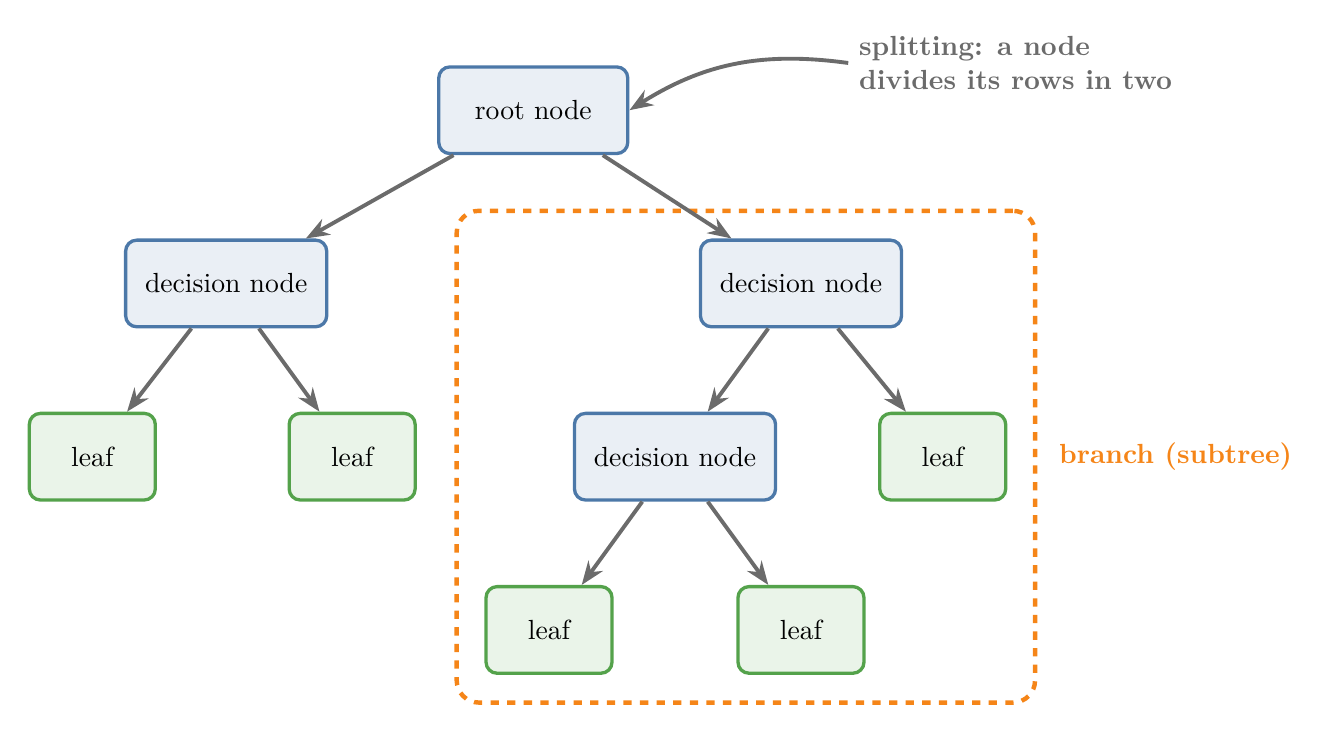
\begin{tikzpicture}[
  q/.style={box=cblue, minimum width=2.4cm},
  leaf/.style={box=cgreen, minimum width=1.6cm},
  lab/.style={font=\sffamily\small, fill=white, inner sep=2pt},
  tag/.style={font=\sffamily\bfseries, text=cgrey}]
  \node[q] (r) at (0,0) {root node};
  \node[q] (d1) at (-3.9,-2.2) {decision node};
  \node[q] (d2) at (3.4,-2.2) {decision node};
  \node[leaf] (l1) at (-5.6,-4.4) {leaf};
  \node[leaf] (l2) at (-2.3,-4.4) {leaf};
  \node[q] (d3) at (1.8,-4.4) {decision node};
  \node[leaf] (l3) at (5.2,-4.4) {leaf};
  \node[leaf] (l4) at (0.2,-6.6) {leaf};
  \node[leaf] (l5) at (3.4,-6.6) {leaf};
  \foreach \a/\b in {r/d1, r/d2, d1/l1, d1/l2, d2/d3, d2/l3, d3/l4, d3/l5} \draw[arrow] (\a) -- (\b);
  \begin{scope}[on background layer]
    \node[draw=corange, dashed, line width=1.6pt, rounded corners=8pt, fit=(d2) (l3) (l4) (l5), inner sep=10pt] (sub) {};
  \end{scope}
  \node[tag, text=corange, anchor=west] at ([xshift=4pt]sub.east) {branch (subtree)};
  \node[tag, anchor=west, align=left] (sp) at (4.0,0.6) {splitting: a node\\divides its rows in two};
  \draw[arrow] (sp.west) to[bend right=20] (r.east);
\end{tikzpicture}
\end{document}
